\subsection{Training set generation}

To build SVM decision function representation from a range image the training set consisting of positive and negative example is necessary. In \cite{SVS2013} the authors work with shape images with white interior and black exterior. The positive examples are sampled from interior and the negative from exterior.

I introduce the range image interior as the part of space between the sensor and obstacles. Conversely, I call the part behind the obstacles exterior. I use the points of the range image as positive examples. The negative examples are obtained by the following algorithm:
\begin{enumerate}
\item
The normals are estimated at all the points of the range image and are oriented away from the sensor.
\item
Each positive example $p^+$ is shifted on the $w_{gap} \cdot \rho_{p^+}$ distance in the normal direction to obtain a new negative example $p_{-}$, where $\rho_{p^+}$ is the distance from $p^+$ to its nearest range image neighbor and $w_{gap}$ is the width of the gap, the algorithm's parameter. This value will be later referred to as \textit{local resolution} of the point cloud, since it is meant to approximate the distance beetween neighboring point of the range image in the vicinity of~$p^+$.
\end{enumerate}
The method is illustrated in the figure \ref{tset}.
\begin{figure}
\centering
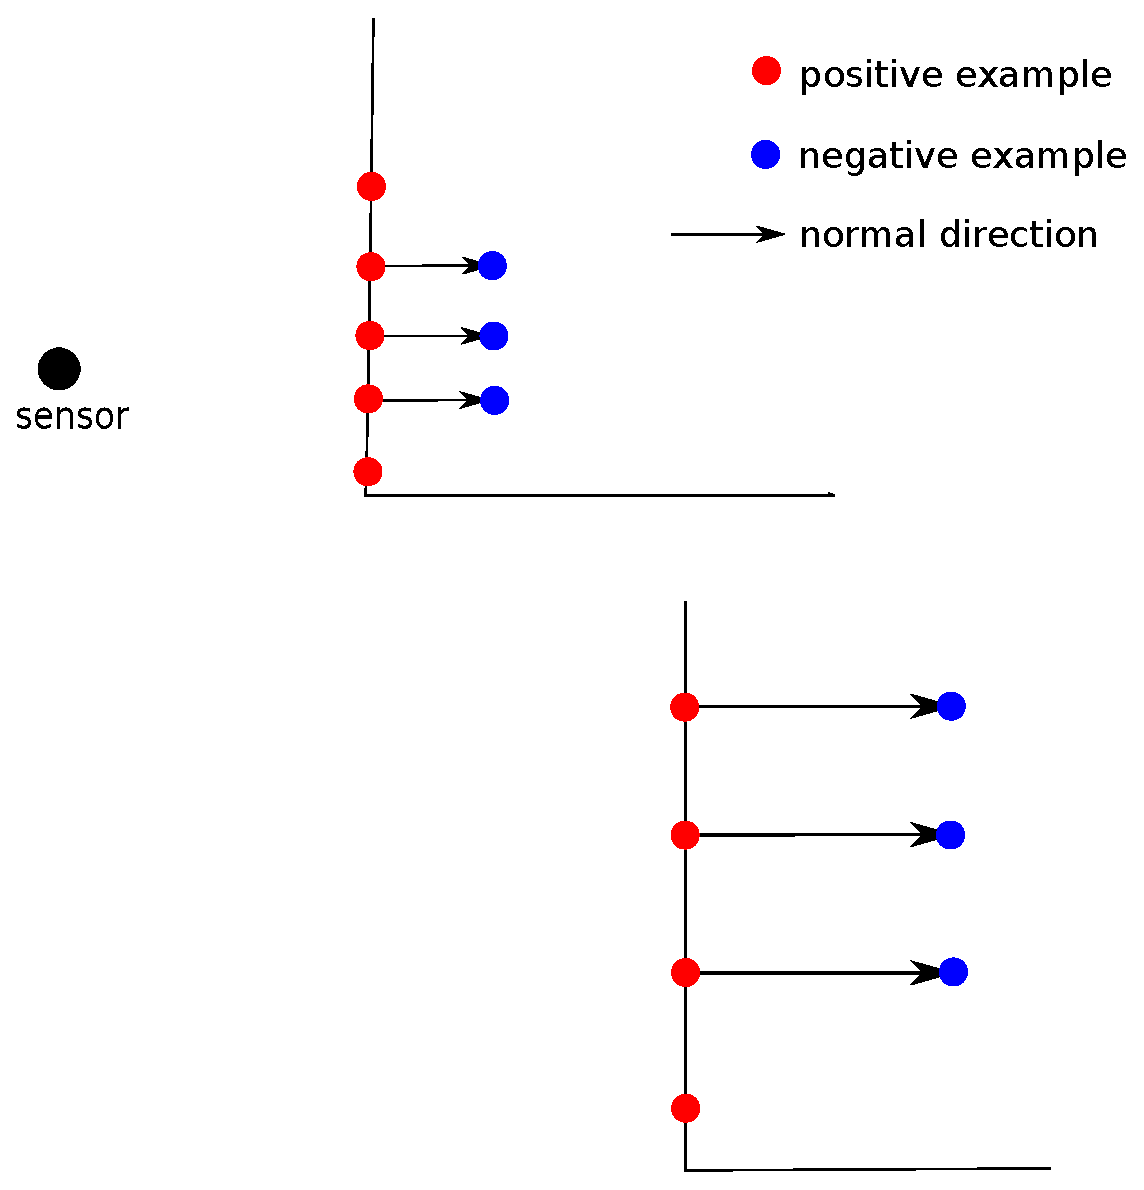
\includegraphics[scale=0.5]{training_set.eps}
\caption{Training set generation. The negative examples are shifted positive examples.}
\label{tset}
\end{figure}

\subsection{Extracting sparse Q structure from range image}
The points of range image are organized in $2D$ grid according to their spatial position. This property allows quick approximate search of all neighbors of given range image point $p$ within given radius~$R$. It is enough to consider the $r$ by $r$ square with the center in $p$, where $r=\Ceil{\frac{R}{\rho_{p}}}$. The points of the square can be than iterated with their distance to $p$ being checked to be less than $R$.

Using this approximate search algorithm the row of the $Q$ can be calculated on request. The modification is necessary to take care of negative examples: they are associated with the point of the range image they are obtained from. The calculated rows are stored in LRU cache, since despite its sparsity the full $Q$ matrix is too large to be stored in main memory. The cache faults are rare and do not impact the performance significantly (see corresponding section).

\subsection{Feature point search}

\subsection{Parameters}
